\section{Pendahuluan}
\subsection{Latar Belakang}
Pada Wireless Jaringan Komputer, terdapat setidaknya 3 jenis, yaitu Point-to-Point Protocol (PPP),
Point-to-multipoint dan Wireless Bridging. 
\\ \\Point-to-Point Protocol (PPP) adalah data link protokol yang umum digunakan dalam membangun 
hubungan langsung antara dua node jaringan. Hal ini dapat menyediakan koneksi otentikasi, transmisi enkripsi (menggunakan ECP, RFC 1968), dan kompresi. 
Jenis ini biasanya digunakan untuk menghubungkan jaringan antar 2 gedung atau antar 2 BTS (Base Transceiver Station).
\\ \\Point-to-multipoint adalah pendekatan yang paling populer untuk komunikasi nirkabel yang memiliki banyak node, tujuan akhir atau pengguna akhir. 
Jenis ini biasanya digunakan untuk membuat wifi atau hotspot yang berasal dari 1 sumber disebar ke banyak client dalam suatu jaringan.
\\ \\Wireless Bridging digunakan untuk menghubungkan dua segmen LAN melalui tautan nirkabel. Kedua
segmen akan berada di subnet yang sama dan terlihat seperti dua switch Ethernet yang dihubungkan
oleh kabel ke semua komputer di subnet.
\\ \\Untuk mengembangkan jaringan komputer berbasis wireless yang berkualitas dan mempunyai ketersediaan tinggi, penggunaan 3 jenis ini perlu disesuaikan dengan kebutuhan dan kondisi nya, sehingga
kali ini saya akan membahasnya 1 persatu dari 3 jenis koneksi wireless tersebut.

\subsection{Maksud dan Tujuan}
Mengetahui dan memahami 3 jenis koneksi pada Jaringan Wireless.
%===========================================================%

\section{Tujuan Praktikum}
Tujuannya apa kamu melakukan praktikum ini
%===========================================================%

\section{Alat dan Bahan}
\begin{itemize}[label=$\bullet$, itemsep=-1pt, leftmargin=*]
	\item paham lah ya isinya
\end{itemize}
%===========================================================%

\section{Langkah-langkah Percobaan}

\subsection{Judul Percobaan 1}
\begin{enumerate}
	\item Konfigurasi router1 dengan ip address 123.656.78.1/24
	\begin{figure}[H]
		\centering
		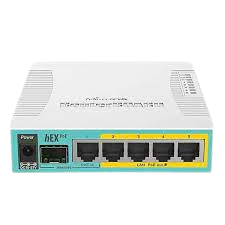
\includegraphics[width=0.5\linewidth]{P1/img/contoh.png}
		\caption{Gambar Contoh}
		\label{fig:gambar1}
	\end{figure}
\end{enumerate}

\subsection{Judul Percobaan 2}
\begin{enumerate}
	\item 
\end{enumerate}
%===========================================================%

\section{Hasil Percobaan}
Hasil dari percobaan yang sudah kamu buat
%===========================================================%

\section{Kesimpulan}
simpulkan
%===========================================================%

\section{Lampiran}
berisi tugas pendahuluan dan dokumentasi saat melakukan praktikum